\documentclass[a4paper,12pt]{article}
\usepackage{xltxtra}

\usepackage{fontspec} 
\defaultfontfeatures{Ligatures={TeX}}   
\setromanfont[
BoldFont=xits-bold.otf,
ItalicFont=xits-italic.otf,
BoldItalicFont=xits-bolditalic.otf,
]{xits-regular.otf}

\usepackage[english,russian]{babel}	
\usepackage{wrapfig}
\usepackage{ccaption}
% заменяем для рисунков ’: ’ после номера рисунка на ’. ’
\captiondelim {. } % после точки стоит пробел !
\usepackage[justification=centering]{caption}
\usepackage{longtable}

\defaultfontfeatures{Ligatures=TeX,Mapping=tex-text}

\addto\captionsrussian{%
    \renewcommand{\figurename}{рис.}%
}

\author{Евгений Деин}
\title{Контрольное задание №4}

\begin{document}
	\maketitle
	\section{Рисунки}

	% рис. 13
	\begin{figure}[h]
        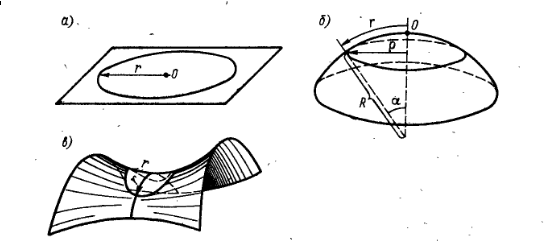
\includegraphics[scale=0.8]{fig_13}
        
        \caption{Окружности \\
        	а — на плоскости (поверхность нулевой гауссовой кривизны); б — иа по-
        	поверхности положительной гауссовой кривизны; в — на поверхности отрица-
        	отрицательной гауссовой кривизны}
        \label{eq:image_13}
	\end{figure}

    % полностью страница 22

    Средняя кривизна поверхности входит в результаты многих и разнообразных механических задач.
    Второй инвариант представляет собой так называемую \textit{гауссову} (или полную) \textit{кривизну} поверхности в данной точке:
    \begin{displaymath}
        K=k_1k_2.
    \end{displaymath}
   

    В зависимости от знаков главных кривизн $k_1$ и $k_2$ можно отметить следующие характерные случаи в исследуемой точке, охватывающие любые ре
    \begin{wrapfigure}[14]{l}{0.67\linewidth}
        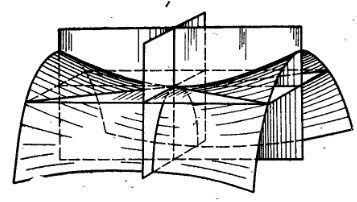
\includegraphics[width=\linewidth]{fig_9}
        \caption{Отрицательная гауссова
            в точке поверхности
            кривизна}
        \label{eq:image_9}
    \end{wrapfigure} гулярные поверхности. 

    
    Если главные кривизны $k_1$ и $k_2$ имеют одинаковые знаки, то кривиз    
    \begin{wrapfigure}{l}{2.2\linewidth}
        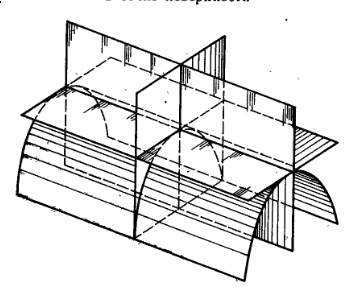
\includegraphics[width=\linewidth]{fig_10}
        \caption{Нулевая гауссова кривизна в точке
            поверхности}
        \label{eq:image_10}
    \end{wrapfigure} на поверхности в исследуемой точке \textit{положительна} и сама поверхность в окрестности этой точки имеет вид, показанный на рис. 7 (индикатриса Дюпена в этом случае — эллипс).
    
    Если главные кривизны $k_1$ и $k_2$ имеют разные знаки, то гауссова кривизна поверхности в исследуемой точке А \textit{отрицательна}, а сама поверхность в окрестности этой точки имеет седлообразный вид, изображенный на рис. \ref{eq:image_9} (индикатриса Дюпена представляет собой
    в этом случае гиперболы).
    
    Если одна из кривизн равна нулю, то гауссова кривизна в ис-
    исследуемой точке А равна \textit{нулю} и поверхность
    в окрестности этой точки имеет вид, изображенный на рис. \ref{eq:image_10} (индикатриса Дюпена представляет собой в этом случае две параллельные прямые).
    
    Наконец, нулю гауссова кривизна может равняться в точке А
    поверхности и в том случае, если обе главные кривизны равны
    нулю. Такие точки называются \textit{точками уплощения}; в их окрестности поверхность имеет сложные свойства.

	\section{Таблицы}
    \subsection{Из картинки}
    \begin{table}[!htp]
        \centering
        \caption{Перевозка бетонных и железобетонных изделий, стеновых и перегородочных материалов(кирпич, блоки, камни, плиты, панели), лесоматериалов круглых и пиломатериалов}
        \label{tab:table1}
        \begin{tabular}{| p{2,5cm} |c|c|c|c|}
            \hline
            \textbf{Расстояние перевозки, км} & \multicolumn{4}{|c|}{Класс груза} \\
            \cline{2-5}
            & \multicolumn{2}{|c|}{\textbf{1}} & \multicolumn{2}{|c|}{\textbf{2}} \\ 
            \cline{2-5}
            & \textbf{на 01.01.200 г.} & \textbf{на 01.03.2005 г.} & \textbf{ на 01.01.2000 г.} & \textbf{на 01.03.2005 г.} \\ \hline
            1 & \textbf{3,28} & 16,19 & \textbf{4,17} & 20,58 \\ 
            \hline
            2 & \textbf{4,17} & 20,58 & \textbf{5,21} & 25,71 \\ 
            \hline
            3 & \textbf{5,21} & 25,71 & \textbf{6,55} & 32,32 \\ 
            \hline
            4 & \textbf{6,26} & 30,89 & \textbf{7,74} & 38,20 \\ 
            \hline
            5 & \textbf{8,19} & 40,42 & \textbf{8,93} & 44,07 \\ 
            \hline
            6 & \textbf{9,22} & 45,50 & \textbf{10,27} & 50,68 \\ 
            \hline
            7 & \textbf{10,13} & 11,17 & \textbf{7,74} & 38,20\\ 
            \hline
            8 & \textbf{12,20} & 60,21 & \textbf{12,20} & 60,21\\ 
            \hline
            9 & \textbf{20,55} & 101,41 & \textbf{7,74} & 38,20\\ 
            \hline
            10 & \textbf{27,24} & 134,43 & \textbf{20,55} & 101,41\\ \hline
            20 & \textbf{ 33,19} & 163,79 &  \textbf{20,55} & 101,41 \\ \hline
            30 & \textbf{40,20} & 189,90 &  \textbf{ 33,19} & 163,79\\ \hline
            40 & \textbf{12,20} & 60,21 & \textbf{12,20} & 60,21\\ 
            \hline
            50 & \textbf{20,55} & 101,41 & \textbf{7,74} & 38,20\\ 
            \hline
            60 & \textbf{27,24} & 134,43 & \textbf{20,55} & 101,41\\ \hline
            70 & \textbf{ 33,19} & 163,79 &  \textbf{20,55} & 101,41 \\ \hline
            80 & \textbf{40,20} & 189,90 &  \textbf{ 33,19} & 163,79\\ \hline
            90 & \textbf{140,20} & 149,90 &  \textbf{ 33,19} & 163,79\\ \hline
            100 & \textbf{112,20} & 340,21 & \textbf{72,20} & 60,21\\ 
            \hline
            110 & \textbf{120,55} & 401,41 & \textbf{98,74} & 38,20\\ 
            \hline
            120 & \textbf{127,24} & 334,43 & \textbf{90,55} & 101,41\\ \hline
        \end{tabular}
    \end{table}

    \subsection{Из файла}
    \begin{longtable}[!hbp]{l p{5cm} p{5cm} p{3cm}}        \caption{Перечень сборников государственных сметных норм на строительные и специальные строительные работы (ГЭСН-2001)}
        \label{tab:table2} \\
        \hline
        \textnumero Сборника	& Наименование сборника	& Полное обозначение сборника	& Сокращенное обозначение сборника \\ \hline
        1 	& Земляные работы							& ГЭСН 81-02-01-2001 	& ГЭСН-2001-01\\ 
        2 	& Горновскрышные работы						& ГЭСН 81-02-02-2001 	& ГЭСН-2001-02\\
        3 	& Буровзрывные работы						& ГЭСН 81-02-03-2001 	& ГЭСН-2001-03\\ 
        4 	& Скважины									& ГЭСН 81-02-04-2001 	& ГЭСН-2001-04\\
        5 	& Свайные работы. Закрепление грунтов. 
        Опускные колодцы						& ГЭСН 81-02-05-2001 	& ГЭСН-2001-05\\
        6 	& Бетонные и железобетонные 
        конструкции монолитные					& ГЭСН 81-02-06-2001 	& ГЭСН-2001-06\\ 
        7	& Бетонные и железобетонные 
        конструкции сборные						& ГЭСН 81-02-07-2001 	& ГЭСН-2001-07\\ 
        8	& Конструкции из кирпича и блоков 			& ГЭСН 81-02-08-2001 	& ГЭСН-2001-08\\ 
        9	& Строительные металлические 
        конструкции 							& ГЭСН 81-02-09-2001 	& ГЭСН-2001-09\\ 
        10 	& Деревянные конструкции					& ГЭСН 81-02-10-2001 	& ГЭСН-2001-10\\ 
        11 	& Полы										& ГЭСН 81-02-11-2001 	& ГЭСН-2001-11\\ 
        12 	& Кровли									& ГЭСН 81-02-12-2001 	& ГЭСН-2001-12\\ 
        13 	& Защита строительных конструкций 
        и оборудования от коррозии				& ГЭСН 81-02-13-2001 	& ГЭСН-2001-13\\ 
        14 	& Конструкции в сельском строительстве		& ГЭСН 81-02-14-2001 	& ГЭСН-2001-14\\ 
        15 	& Отделочные работы							& ГЭСН 81-02-15-2001 	& ГЭСН-2001-15\\ 
        16 	& Трубопроводы внутренние					& ГЭСН 81-02-16-2001 	& ГЭСН-2001-16\\ 
        17 	& Водопровод и канализация --- 
        внутренние устройства					& ГЭСН 81-02-17-2001 	& ГЭСН-2001-17\\ 
        18 	& Отопление --- внутренние устройства		& ГЭСН 81-02-18-2001 	& ГЭСН-2001-18\\ 
        19 	& Газоснабжение --- внутренние устройства	& ГЭСН 81-02-19-2001 	& ГЭСН-2001-19\\ 
        20 	& Вентиляция и кондиционирование воздуха	& ГЭСН 81-02-20-2001 	& ГЭСН-2001-20\\
        21 	& Временные сборно-разборные здания 
        и сооружения							& ГЭСН 81-02-21-2001 	& ГЭСН-2001-21\\ 
        22 	& Водопровод --- наружные сети				& ГЭСН 81-02-22-2001 	& ГЭСН-2001-22\\ 
        23 	& Канализация --- наружные сети				& ГЭСН 81-02-23-2001 	& ГЭСН-2001-23\\ 
        24 	& Теплоснабжение и газопроводы				& ГЭСН 81-02-24-2001 	& ГЭСН-2001-24\\ 
        25 	& Магистральные и промысловые трубопроводы	& ГЭСН 81-02-25-2001 	& ГЭСН-2001-25\\ 
        26 	& Теплоизоляционные работы					& ГЭСН 81-02-26-2001 	& ГЭСН-2001-26\\ 
        27 	& Автомобильные дороги						& ГЭСН 81-02-27-2001 	& ГЭСН-2001-27\\ 
        28 	& Железные дороги							& ГЭСН 81-02-28-2001 	& ГЭСН-2001-28\\ 
        29 	& Тоннели и метрополитены					& ГЭСН 81-02-29-2001 	& ГЭСН-2001-29\\ 
        30 	& Мосты и трубы								& ГЭСН 81-02-30-2001 	& ГЭСН-2001-30\\ 
        31 	& Аэродромы									& ГЭСН 81-02-31-2001 	& ГЭСН-2001-31\\ 
        32 	& Трамвайные пути							& ГЭСН 81-02-32-2001 	& ГЭСН-2001-32\\ 
        33 	& Линии электропередачи						& ГЭСН 81-02-33-2001 	& ГЭСН-2001-33\\ 
        34 	& Сооружения связи, радиовещания 
        и телевидения							& ГЭСН 81-02-34-2001 	& ГЭСН-2001-34\\ 
        35 	& Горнопроходческие работы					& ГЭСН 81-02-35-2001 	& ГЭСН-2001-35\\ 
        36 	& Земляные конструкции гидротехнических 
        сооружений								& ГЭСН 81-02-36-2001 	& ГЭСН-2001-36\\ 
        37 	& Бетонные и железобетонные конструкции 
        гидротехнических сооружений				& ГЭСН 81-02-37-2001 	& ГЭСН-2001-37\\ 
        38 	& Каменные конструкции гидротехнических 
        сооружений								& ГЭСН 81-02-38-2001 	& ГЭСН-2001-38\\ 
        39 	& Металлические конструкции 
        гидротехнических сооружений				& ГЭСН 81-02-39-2001 	& ГЭСН-2001-39\\ 
        40 	& Деревянные конструкции гидротехнических 
        сооружений								& ГЭСН 81-02-40-2001 	& ГЭСН-2001-40\\ 
        41 	& Гидроизоляционные работы в 
        гидротехнических сооружениях			& ГЭСН 81-02-41-2001 	& ГЭСН-2001-41\\ 
        42 	& Берегоукрепительные работы				& ГЭСН 81-02-42-2001 	& ГЭСН-2001-42\\ 
        43 	& Судовозные пути стапелей и слипов			& ГЭСН 81-02-43-2001 	& ГЭСН-2001-43\\ 
        44 	& Подводностроительные (водолазные) работы	& ГЭСН 81-02-44-2001 	& ГЭСН-2001-44\\ 
        45 	& Промышленные печи и трубы					& ГЭСН 81-02-45-2001 	& ГЭСН-2001-45\\ 
        46 	& Работы по реконструкции зданий 
        и сооружений							& ГЭСН 81-02-46-2001 	& ГЭСН-2001-46\\ 
        47 	& Озеленение. Защитные лесонасаждения		& ГЭСН 81-02-47-2001 	& ГЭСН-2001-47\\ 
        48 	& Скважины на нефть и газ					& ГЭСН 81-02-48-2001 	& ГЭСН-2001-48\\ 
        49 	& Скважины на нефть и газ 
        в морских условиях						& ГЭСН 81-02-49-2001 	& ГЭСН-2001-49\\ 
    \end{longtable}	
\end{document}